\newpage

\subsubsection{UCA 4 - Inserimento modalità di tracciamento}%kite level

\begin{figure}[h]
	\centering	
	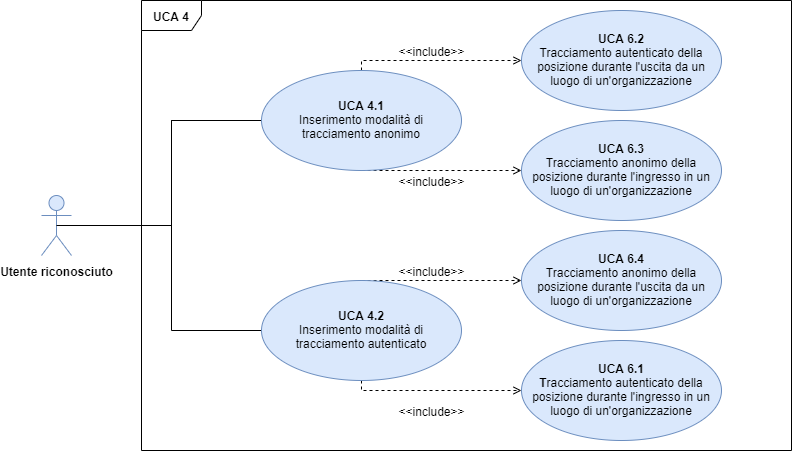
\includegraphics[scale=0.53]{sezioni/UseCase/Immagini/UCA4.png}
	\caption{UCA 4 - Inserimento modalità di tracciamento}
\end{figure}

\begin{itemize}
	\item \textbf{Attori primari:} Utente riconosciuto;
	\item \textbf{Precondizione:} L'utente si è autenticato con le credenziali LDAP\ap{G} nella organizzazione in cui si trova e vuole selezionare la modalita di tracciamento;
	\item \textbf{Postcondizione:} L'utente viene tracciato secondo la modalità da lui scelta precedentemente; 
	\item \textbf{Scenario principale:} L'utente accede alla funzionali di "Inserimento modalità di tracciamento";
	\item \textbf{Flusso di eventi:}
	\begin{itemize}
		\item UCA 4.1 - Inserimento modalità anonimo\ap{G};
		\item UCA 4.2 - Inserimento modalità autenticato\ap{G}.
	\end{itemize}
\end{itemize}

\subsubsection{UCA 4.1 - Inserimento modalità anonimo}%sea level
\begin{itemize}
\item \textbf{Attori primari:} Utente riconosciuto;
\item \textbf{Precondizione:} L'utente si è autenticato con le credenziali LDAP\ap{G} nella organizzazione in cui si trova e vuole selezionare la modalità di tracciamento anonimo\ap{G}];
\item \textbf{Postcondizione:}  L'utente viene tracciato secondo la modalità anonimo;
\item \textbf{Flusso di Eventi:}
	\begin{itemize}
	%Queste devono diventare UCA 4.1.1 e 4.1.2 e avere una loro sezione apposta 
	%\item UCA 4.1.1 - L'utente accede alla funzionalità inserimento modalità di tracciamento;  -----> Tipo così
	\item L'utente accede alla funzionalità inserimento modalità di tracciamento; 
	\item L'utente inserisce la modalità anonimo.
\end{itemize}
\end{itemize}

\subsubsection{UCA 4.2 - Inserimento modalità autenticato}%sea level
\begin{itemize}
	\item \textbf{Attori primari:} Utente riconosciuto;
	\item \textbf{Precondizione:} L'utente si è autenticato con le credenziali LDAP\ap{G} nella organizzazione in cui si trova e vuole selezionare la modalita di tracciamento autenticato\ap{G};
	\item \textbf{Postcondizione:}  L'utente viene tracciato secondo la modalità autenticato;
	\item \textbf{Flusso di eventi:}
	\begin{itemize}
	%Queste devono diventare UCA 4.2.1 e 4.2.2 e avere una loro sezione apposta 
		\item L'utente accede alla funzionalità inserimento modalità di tracciamento;
		\item L'utente inserisce la modalità autenticato.
	\end{itemize}
\end{itemize}
